\section{Efficiency calculations}
\label{sec:hhh:eff}


These efficiencies were calculated using simulated events; therefore, in order that the above
efficiencies are correct it is imperitive that the simulated events describe the data accurately.
Where there are discrepancies, the simulations must be corrected.
There are some variables which are known to be poorly described in simulation, particularly track
multiplicity and the \chisqvtx of the \Bp candidate.
The effects of these discrepancies are minimalised by reweighting simulated events using
the distributions of \btojpsikpipi.
Track multiplicity is known to be poorly described in simulation, generally the number of tracks is
less than in data, these discrepancies are illustrated in \Fig{fig:hhh:ntracks}.
Aside from the direct differencies, the low track multiplicity of in sumulated events is a
contributing factor of PID variables being badly described in simulations.

\begin{figure}
  \begin{center}
    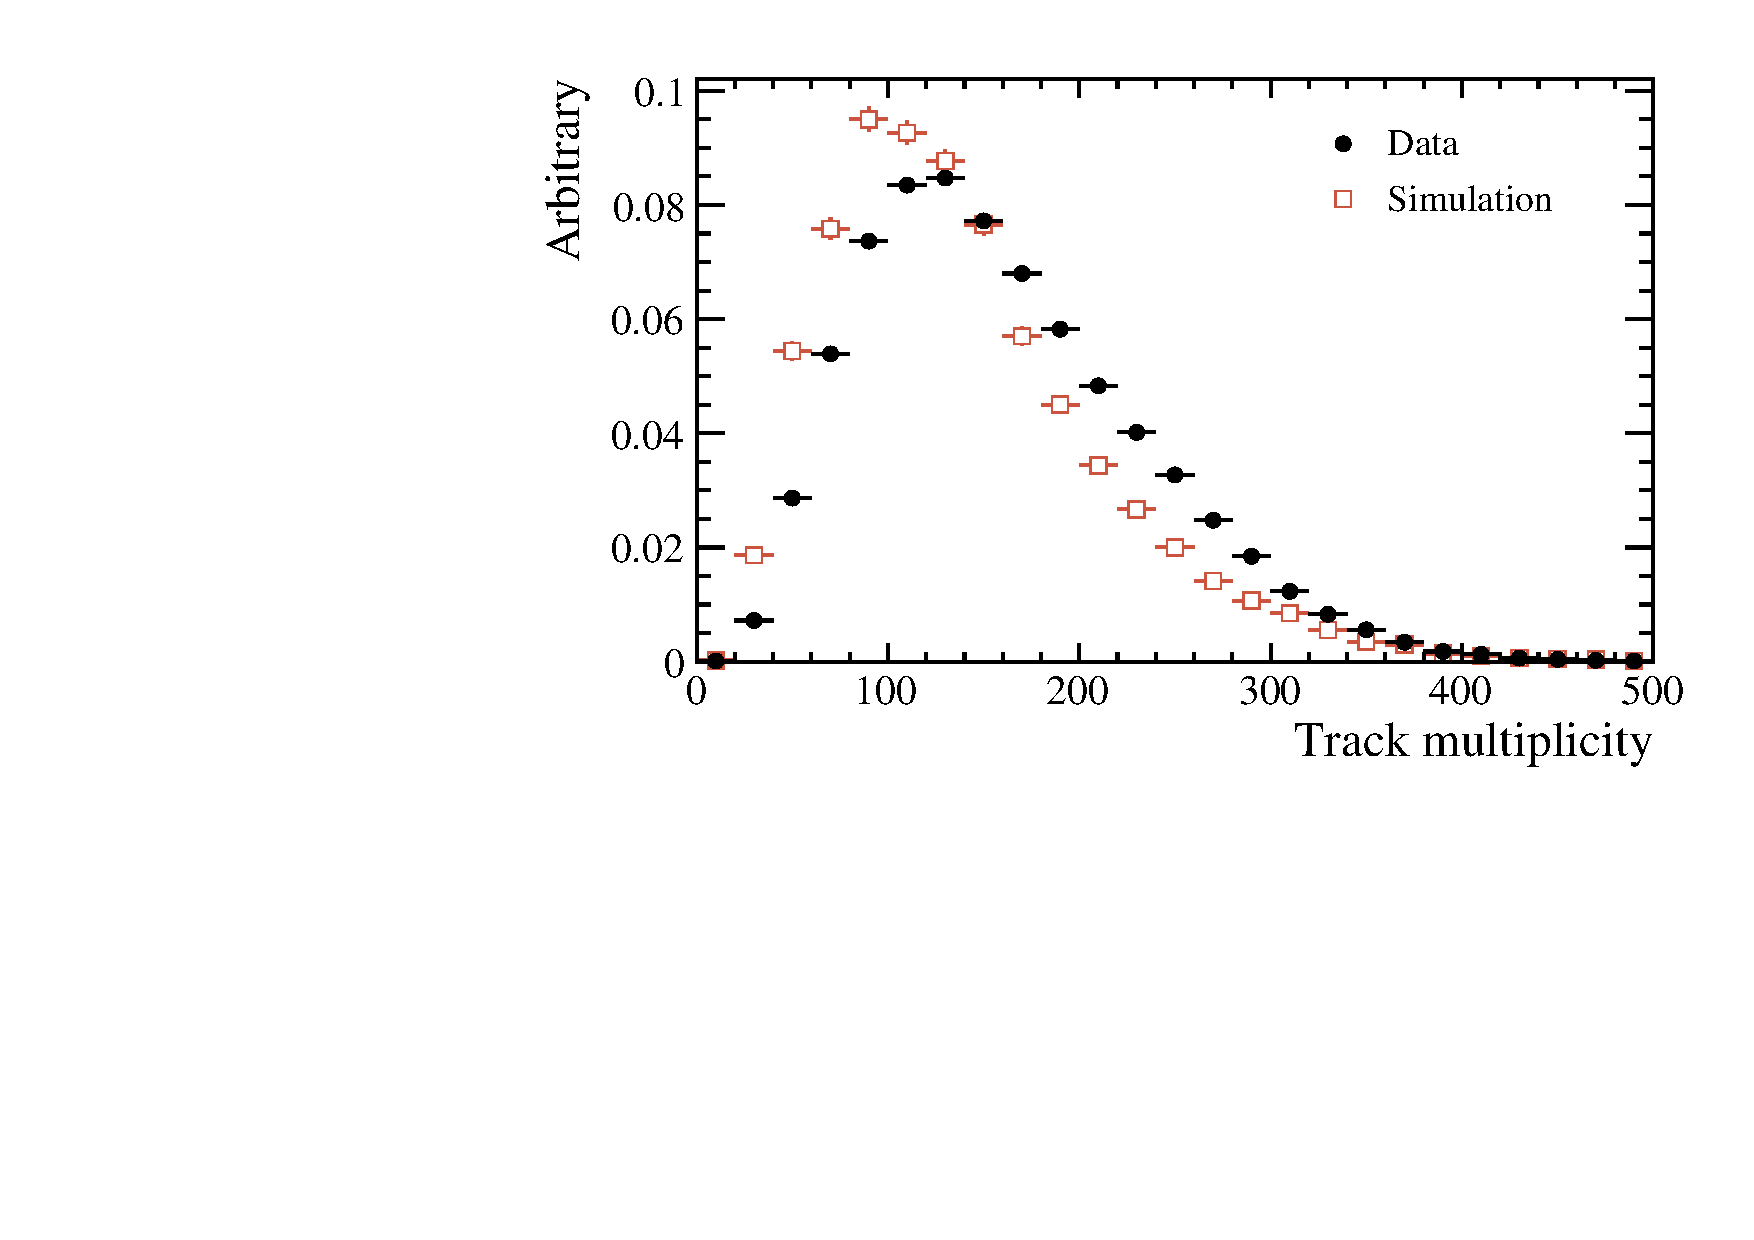
\includegraphics[width=0.48\textwidth]{ntracks}
    \caption[Differences between track multiplicity in data and simulation]
    {\small
      Distributions of track multiplicity for (black circles) data and (red squares) simulation.
      Simulated events are known to mis-model the track multiplicity, having a lower average number
      of tracks per event.
    }
    \label{fig:hhh:ntracks}
  \end{center}
\end{figure}

To ensure that efficiencies from PID cuts are determined accurately from simulation, the variables
must be corrected.
This is done with data driven methods, using highly pure samples of pions, kaons
and muons (which came from the decays \decay{\Dstarp}{\Dz\pip}, where \decay{\Dz}{\Km\pip}, and
\jpsitomumu).
For each track in the simulated \Bp candidate, a new PID variable is rasampled from PID
distributions of the pure track samples as a function of the track's $\eta$, $p$ and track
multiplicity.
Only required for kaons and pions, the muon PID distribution is well described in simulation.
Figure~\ref{fig:hhh:pid} shows the effect of this resampling technique, it is observed that the
simulated PID distributions that have been resampled matches data distributions much more than the
raw distributions; the differences that remain are accounted for in the systematic uncertainties.

\begin{figure}
  \begin{center}
    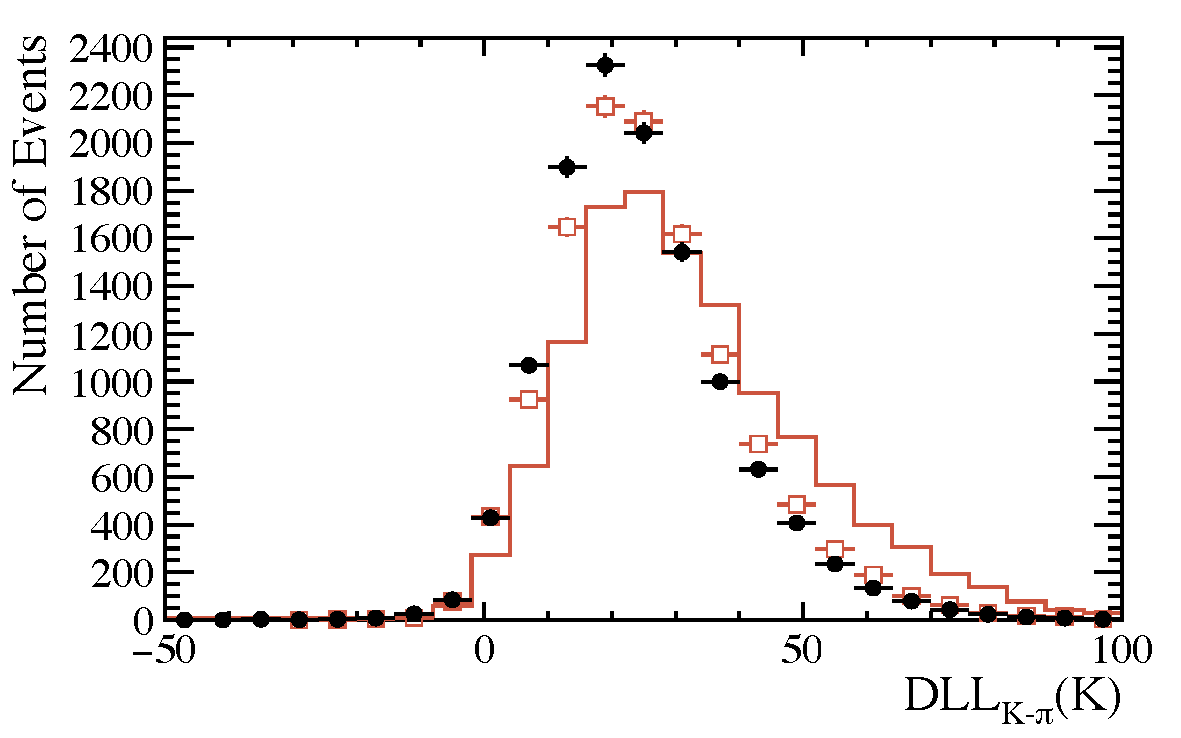
\includegraphics[width=0.48\textwidth]{pid_Kplus}
    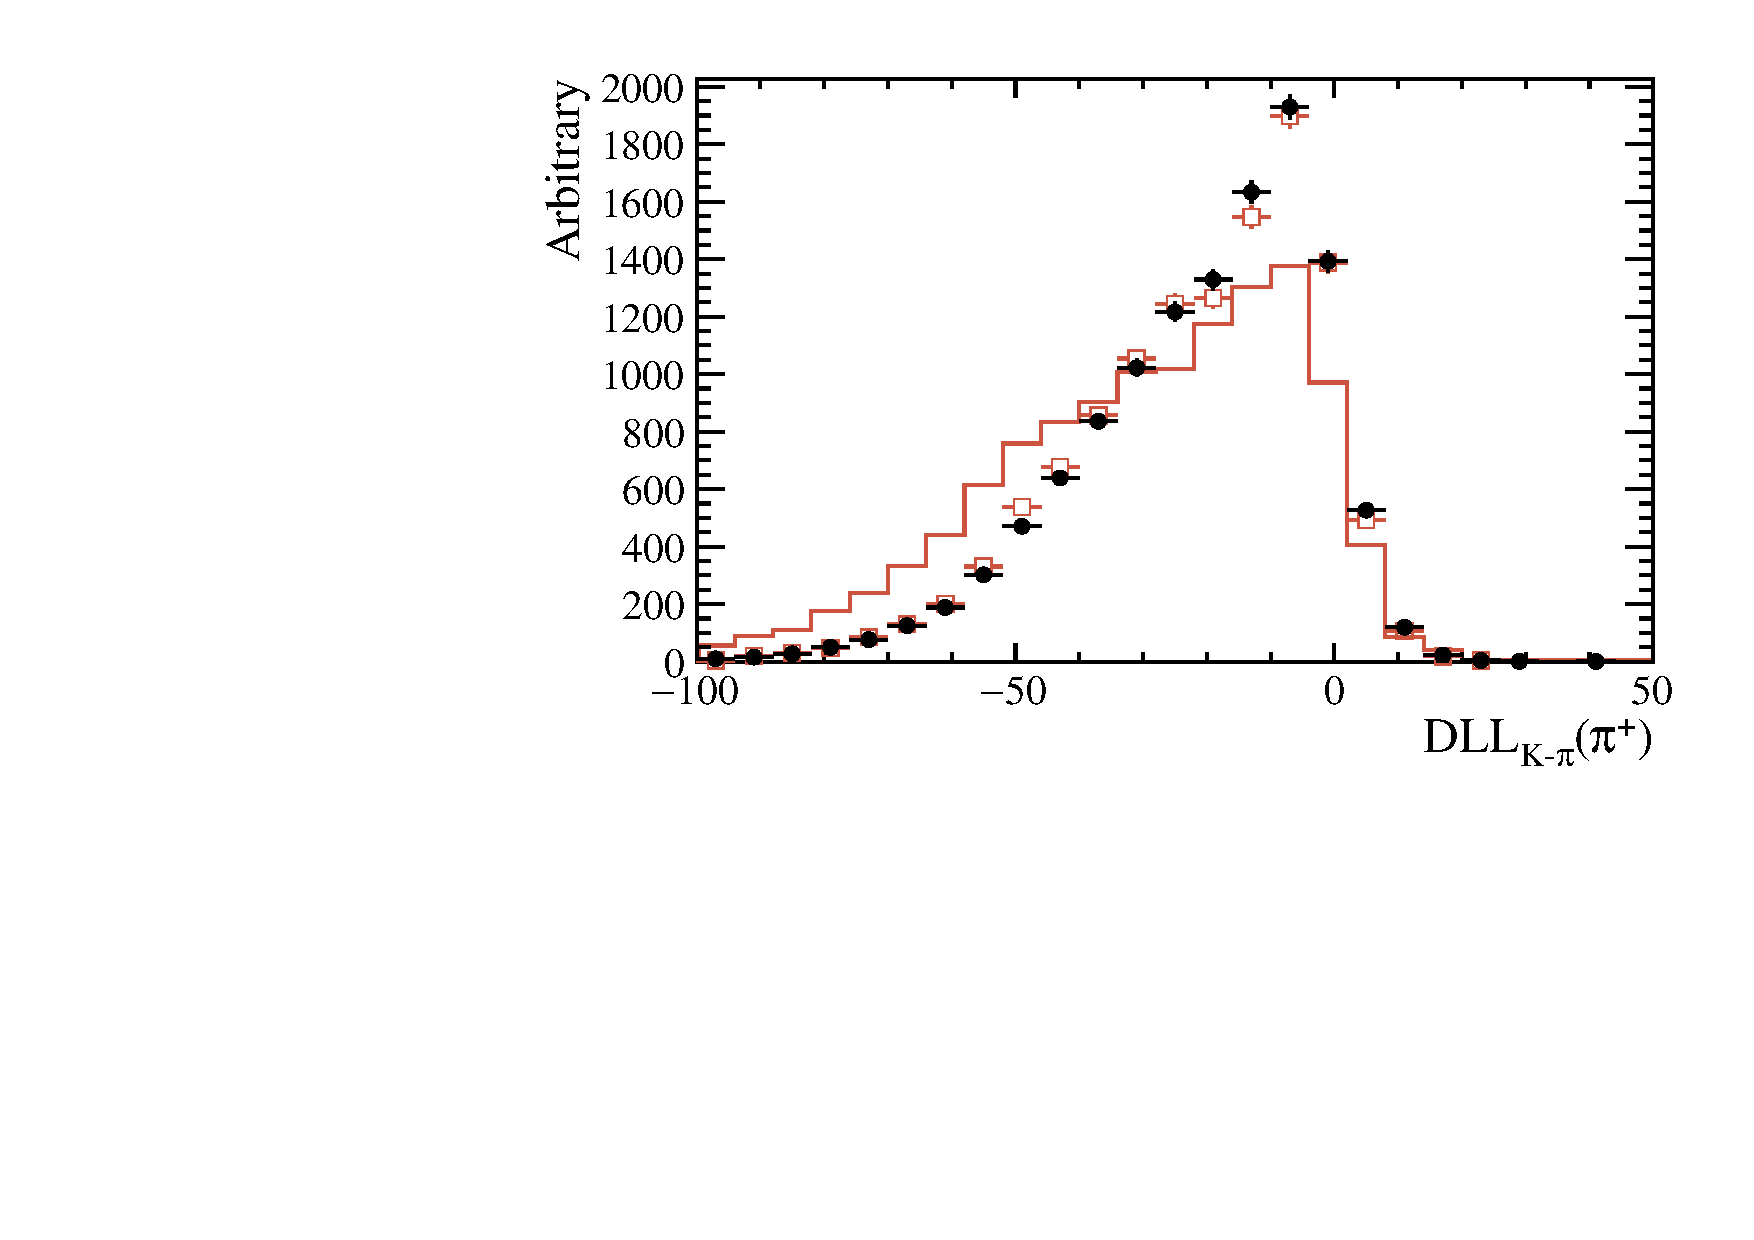
\includegraphics[width=0.48\textwidth]{pid_piplus}\\
    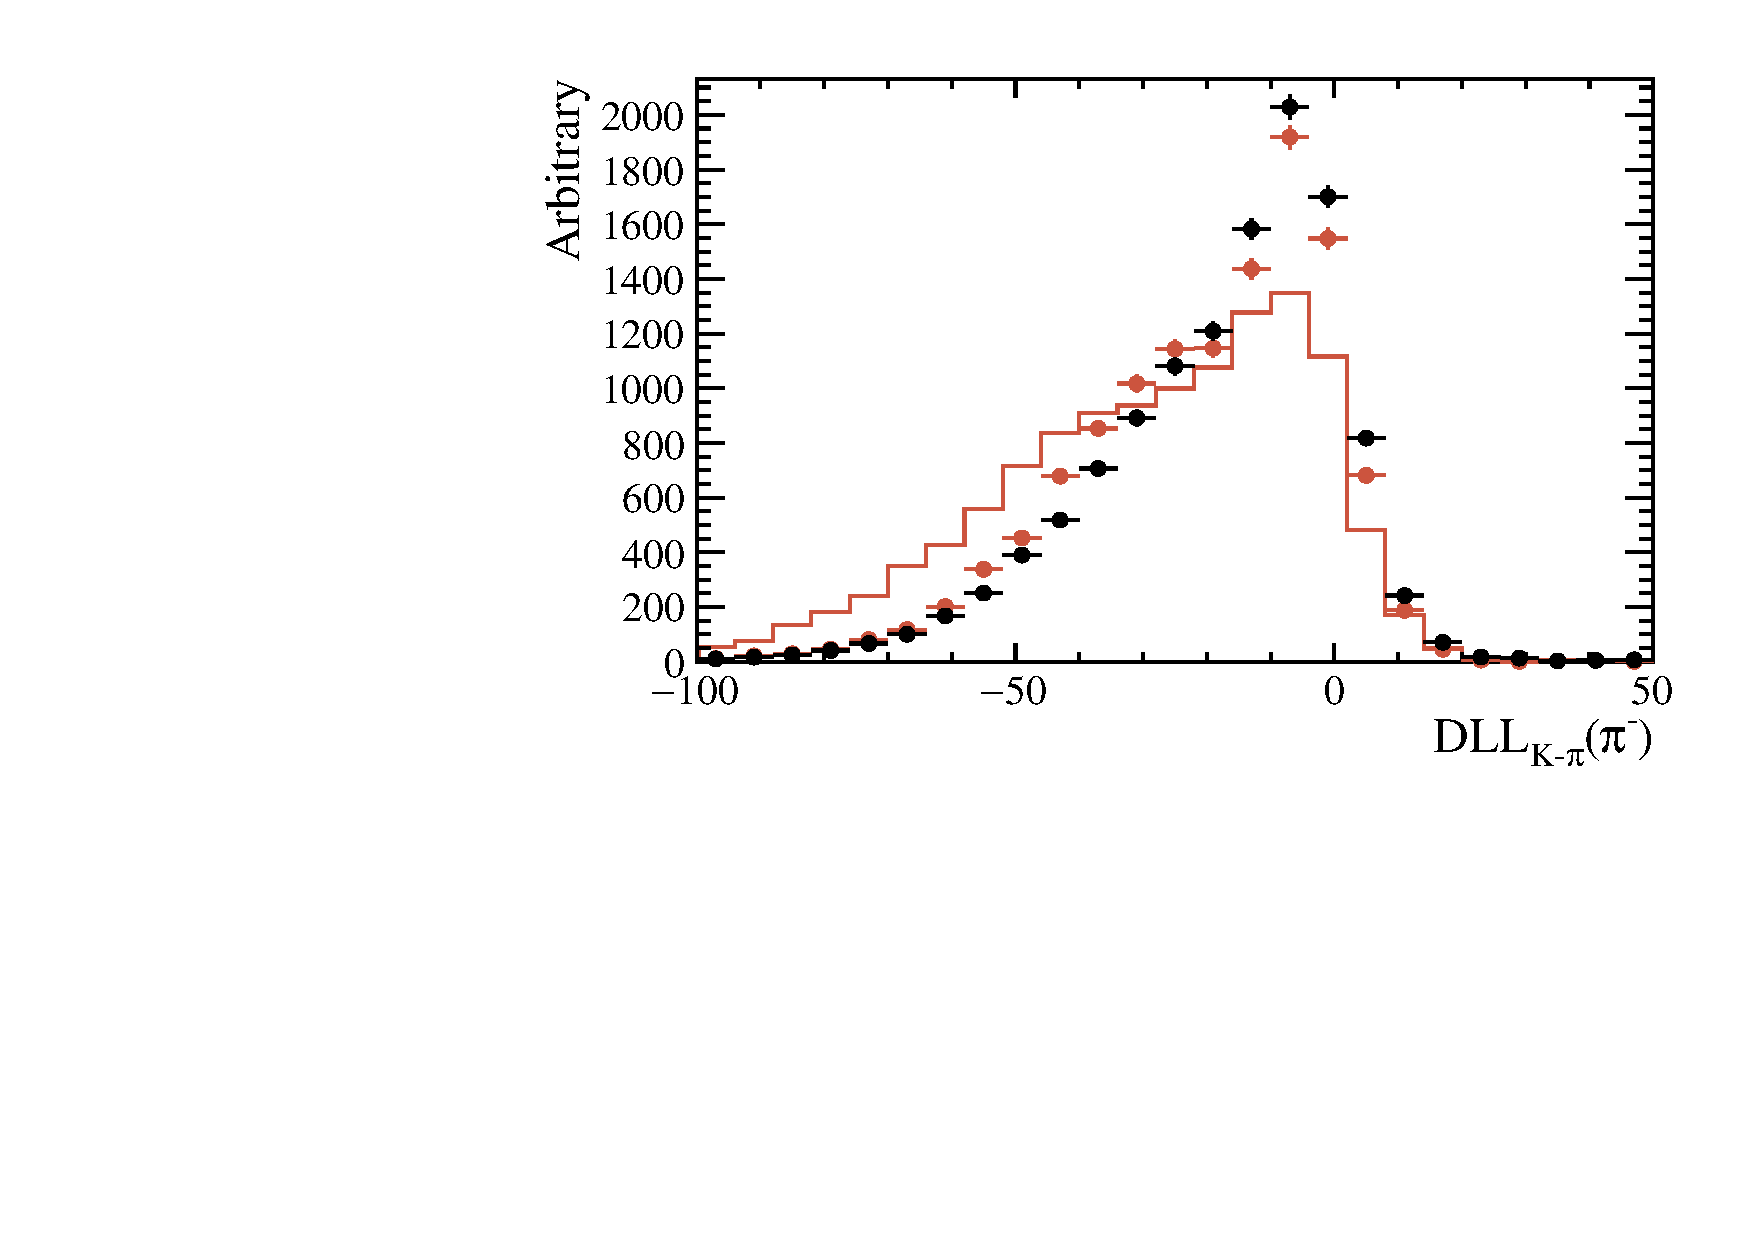
\includegraphics[width=0.48\textwidth]{pid_piminus}
    \caption[Effect of resampling PID variables in simulation]
    {\small
      The effect of PID resampling for simulated tracks using pure samples of pions, kaons and
      muons.
      There is marked improvement in the similarity of the (black circles) \btojpsikpipi data and
      simulated events before (red line) resampling and after (red squares).
    }
    \label{fig:hhh:pid}
  \end{center}
\end{figure}

%Reweighting

Tracking efficiency varies depending upon the regions of the detector through which the paricle
passes, and the modelling of the detector in the simultion behaves differently to in actualoty.
To correct for this, each candidate is weighted based on the relavtive treacking effeciency between
data and simulation, this is dependent upon $m$ and $\eta$.
The same is true for the responce of the {\tt isMuon} variable.
After all rewighting all the aforementioned varialbes in simulated events, the BDT distributions
are seen to be in agreement, this is shown in \Fig{fig:kpipi:bdt}.
%Geometric efficiencies
%Tracking efficiencies and isMuon
%Geometric efficiencies

\begin{figure}
  \begin{center}
    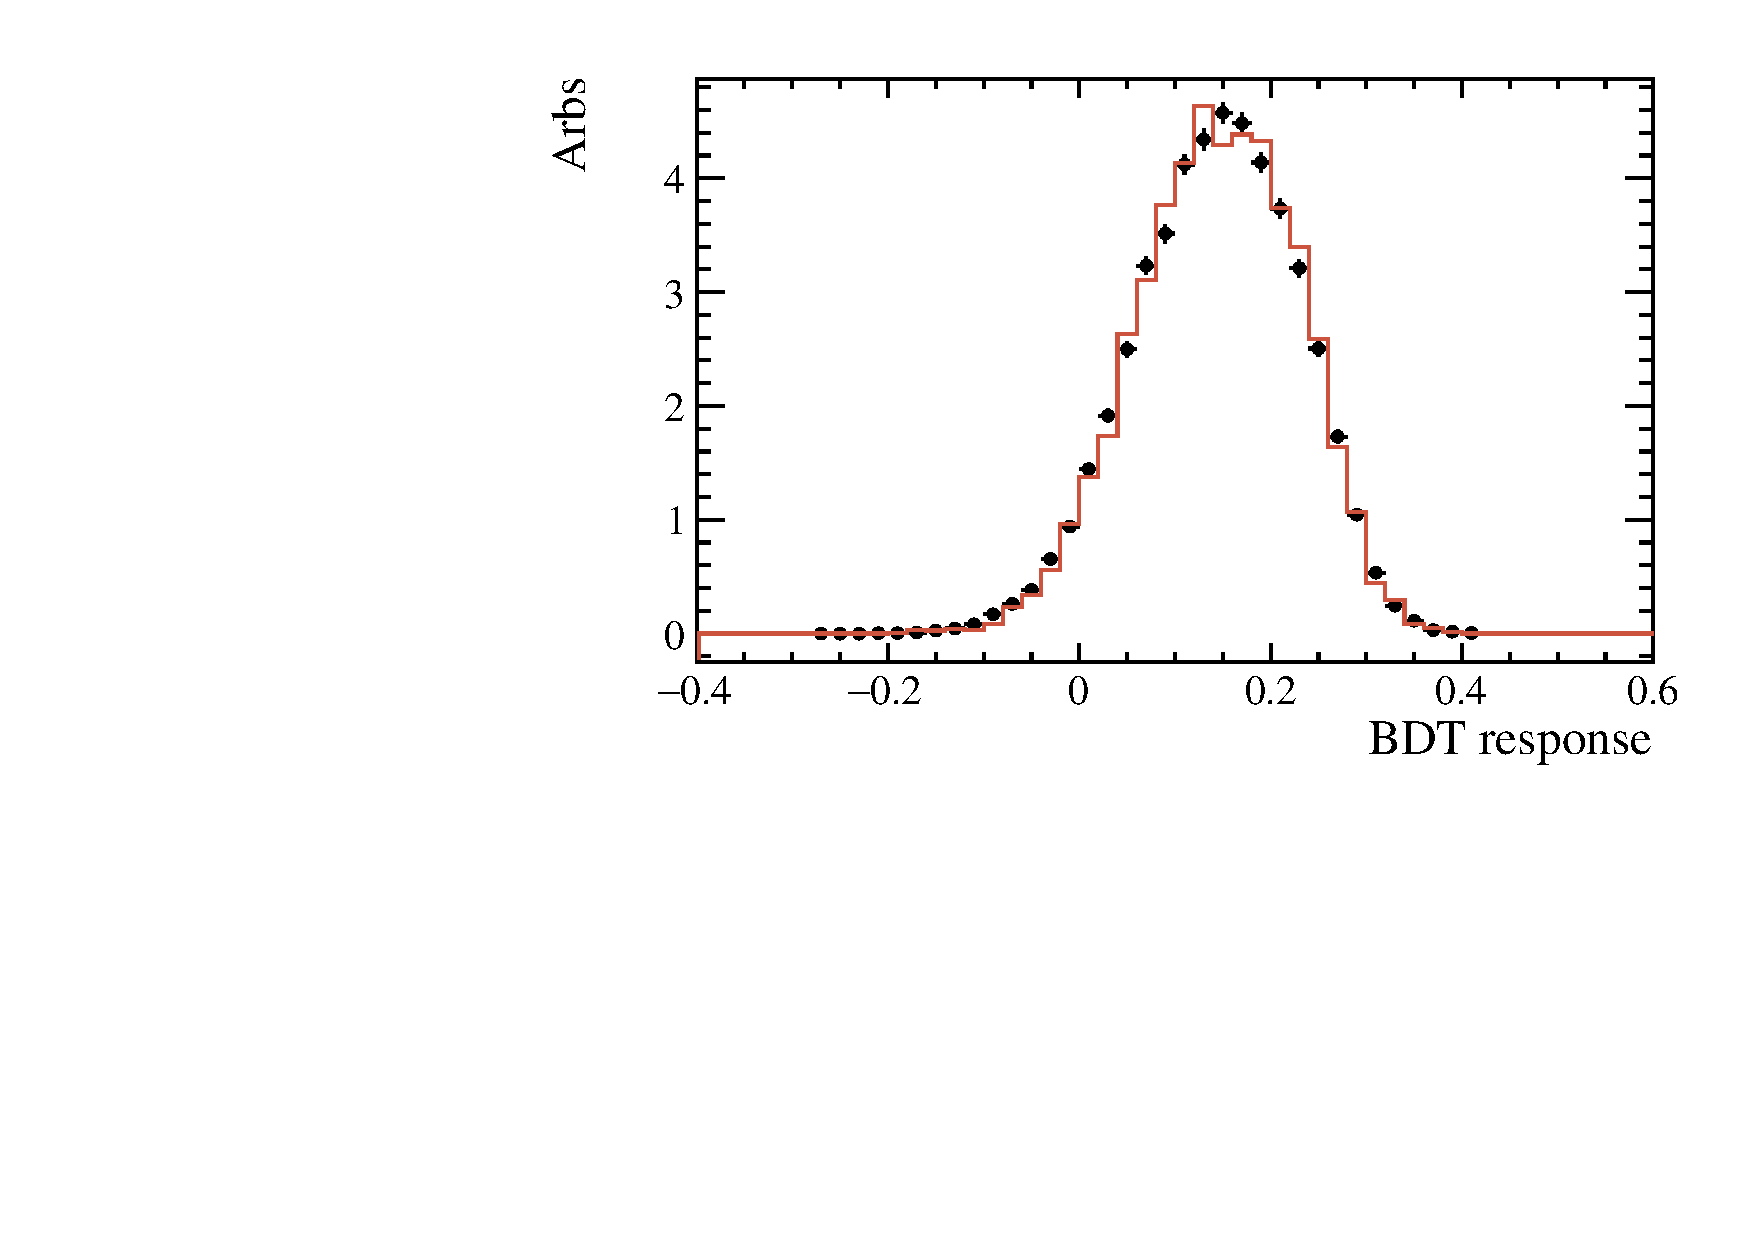
\includegraphics[width=0.48\textwidth]{bdt_k1jpsi}
    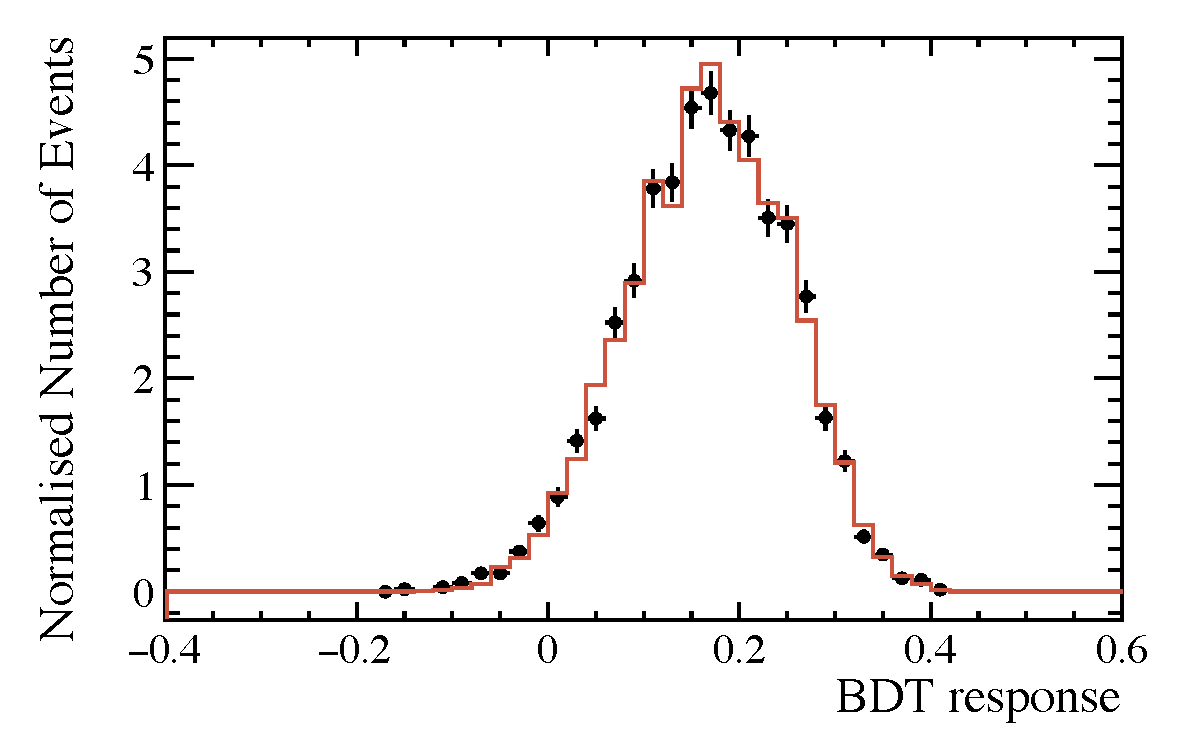
\includegraphics[width=0.48\textwidth]{bdt_psi2sk}
    \caption[BDT distributions in data and simulation]
    {\small
      Distributions of the BDT for data (black points) and simulation (red line) for the decay
      (left) \decay{\Bp}{\jpsi\kone{1270}}
      (right) \btopsitwosk.
    }
    \label{fig:kpipi:bdt}
  \end{center}
\end{figure}

\bam{MAKE A PLOT OF TABLES...}

Once the simulation has been corrected, the total efficincy, \eff{tot} was calculated for each
normalization and signal mode using simulated events.
The value for \eff{tot} is calculated to be $\eff{geo}\eff{reco\&sel}\eff{trig}$, where:
\eff{geo} is the geometric efficiency;
\eff{reco\&sel} is the reconstruction and selection efficiency;
\eff{trig} trigger efficiency.
The Geometric efficiency defines the probability that a \Bp decays into daughter particles which
all pass through the \lhcb detector volume.

%relating to the probabliity of all tracks passing throught the \lhcb dectecor volume;
%Efficiencies for the normalization modes
%$\eff{reco\&sel\&trig}(\btopsitwosk)=(0.4123\pm0.0026)\,\%$, and
%$\eff{reco\&sel\&trig}(\btojpsiphik)=(2.1121\pm0.0013)\,\%$, are calculated


%$\eff{tot}(\btokpipimumu)$,
%$\eff{tot}(\btophikmumu)$, and
%must be made in order to determine the branching fractions for the decays \btokpipimumu and
%\btophikmumu.

%For the decays \btopsitwosk and \btojpsiphik the physics models are well defined, and simulation of
%these events is strainghtforward.
%However, the lack of a model for the inclusive decay \btokpipimumu necessitates an approximation
%must be made with regards to decay model.
%An appropriate choice is the physics model where the \kpipi comes via the \kone{1270} resonance,
%from \Ref{Hatanaka:2008gu} and $\thetakone=34^\circ$.


Since, efficiency calculations require reliable simulated samples of decays, reliable physics
models must be used.
This raises a dilemma deciding how to calculate the efficincy of the signal decays \btokpipimumu
and \btophikmumu, because no physics models exist for them.
For the decay \btokpipimumu, an appropriate choice
was the physics model for \decay{\Bp}{\kone{1270}\mumu}
from \Ref{Hatanaka:2008gu} and $\thetakone=34^\circ$, because this was assumed to be a dominant
contribution.
A phasespace model is used for the signal decay \btophikmumu.
These models introduce systematic uncertainties, which are discussed in \Sec{ssec:kpipi:syst} and
\Sec{ssec:phik:syst}.



